\newcommand{\institut}{Institut f\"ur Energie und Automatisiertungstechnik}
\newcommand{\fachgebiet}{Elektronische Mess- und Diagnosetechnik}
\newcommand{\veranstaltung}{Praktikum Messdatenverarbeitung}
\newcommand{\pdfautor}{Dirk Babendererde (321 836), Thomas Kapa (325 219), Magdalene Busuru (319 433)}
\newcommand{\autor}{Dirk Babendererde (321 836)\\ Thomas Kapa (325 219)\\ Magdalene Busuru (319 433)}
\newcommand{\pdftitle}{Praktikum Messdatenverarbeitung Termin 3}
\newcommand{\prototitle}{Praktikum Messdatenverarbeitung \\ Termin 3}
\newcommand{\aufgabe}{}


\newcommand{\gruppe}{Gruppe: G2 Fr 08-10}
\newcommand{\betreuer}{Betreuer: J\"urgen Funk}


\input{../../../packages/tu_header_8}



% \lstlistoflistings
\definecolor{darkgray}{rgb}{0.95,0.95,0.95}
\definecolor{darkolivegreen}{HTML}{01a801}
\definecolor{functionsBlue}{HTML}{32b9b9}
\definecolor{variableRed}{rgb}{1,0,0}
\definecolor{stringBrown}{HTML}{bc8e8e} % f geht nicht

\lstset{
        %\lstset{extendedchars=true} % Umlaute an der richtigen stelle und nicht am Anfang ausgeben
        %basicstyle=\footnotesize\ttfamily,
        basicstyle=\small,
        %
        inputencoding=utf8,
        %
        tabsize=4,
        showspaces=false,
        showtabs=false,
        showstringspaces=true, % no special string spaces
        %
        backgroundcolor=\color{darkgray}, % background
        stringstyle=\color{stringBrown}\fseries, % Strings
        keywordstyle=\color{functionsBlue}\bfseries, % keywords Blau
        identifierstyle=\color{variableRed}, % variablen
        commentstyle=\color{darkolivegreen}, %  comments
        %
        breaklines=true,
        %
        numbers=left,
        numberstyle=\tiny,
        stepnumber=1,
        numbersep=7pt,
        %
        frame=single,
        columns=flexible,
        %
        xleftmargin=-2cm,
        xrightmargin=-1.5cm,
        %
        language=Matlab,
}
% enables UTF-8 in source code: (dirty, dirty hack)
\lstset{literate=
    %Deutsch
    {ä}{{\"a}}1 {ö}{{\"o}}1 {ü}{{\"u}}1 {Ä}{{\"A}}1 {Ö}
    {{\"O}}1 {Ü}{{\"U}}1 {ß}{\ss}1
    %Türkisch
    {â}{{\^{a}}}1 {Â}{{\^{A}}}1 {ç}{{\c{c}}}1 {Ç}{{\c{C}}}1 {ğ}{{\u{g}}}1 {Ğ}{{\u{G}}}1 {ı}{{\i}}1 {İ}{{\.{I}}}1 {ö}{{\"o}}1 {Ö}{{\"O}}1 {ş}{{\c{s}}}1
    {Ş}{{\c{S}}}1 {ü}{{\"u}}1 {Ü}{{\"U}}1
    %Polish
    {ą}{{\k{a}}}1 {ć}{{\'c}}1 {ę}{{\k{e}}}1 {ł}{{\l{}}}1 {ń}{{\'n}}1 {ó}{{\'o}}1 {ś}{{\'s}}1 {ż}{{\.z}}1 {ź}{{\'z}}1 {Ą}{{\k{A}}}1 {Ć}{{\'C}}1
    {Ę}{{\k{E}}}1 {Ł}{{\L{}}}1 {Ń}{{\'N}}1 {Ó}{{\'O}}1 {Ś}{{\'S}}1 {Ż}{{\.Z}}1 {Ź}{{\'Z}}1
    %Spanish
    {á}{{\'a}}1 {é}{{\'e}}1 {í}{{\'i}}1 {ó}{{\'o}}1 {ú}{{\'u}}1 {ñ}{{\~n}}1
}

%     \lstinputlisting{./praktikum6.sce}

%---------------------------------------------------------------------
%---------------------------------------------------------------------
%---------------------------------------------------------------------

\section{Vorbereitungsaufgaben}


\bq

Eine digitale Messkette besteht aus einem Sensor, der Signalkonditionung (z.B.
Linearisierung, Verstärkung \ldots), dem Antialiasingfilter, einem Abtast- und
Halteglied und einem Analog-Digital-Umsetzer.
Der Analog-Digital-Umsetzer hat eine minimale Abtastfrequenz, z.B. dadurch, dass
man ein Register als Referenz für einen Timer nutzt, dass aber eine begranzte
Anzahl an Bits zur Verfügung stellt.
Sensor, Signalkonitionierung und Antialiasingfilter sitzen in der Wandlerbox,
Abtast- und Haltglied und ADU sitzen auf dem Microcontroller.
\eq

\section{Vorbereitung}
\begin{quote}
    
    \subsection{Tiefpassfilter 2. Ordnung}
    \begin{quote}
        
        Um die Dämpfung bestimmen zu können muss zunächst das $U_{LSB}$ errechnet werden:
        \begin{equation}
    	\begin{split}
    		U_{LSB} = \frac{14V}{2^{10} - 1 Bit} = \frac{14V}{1023 Bit}
    	\end{split}
        \end{equation}
        
        Die Dämpfung ergibt sich nun daraus, dass ab der Grenzfrequenz die Maximale Eingangsspannung von $\pm 7V$ auf unter
        $U_{LSB}/2$ gedämpft werden muss:
        
        
        \begin{equation}
    	\begin{split}
    		A = \frac{14}{7 \p 2} \p \frac{1}{1023} = \frac{1}{1023} = -60 dB
    	\end{split}
        \end{equation}
        
        
        Nun simulieren wir einen Butterworth-Tiefpass 2. Ordnung und lesen ab, bei welcher Frequenz die Amplitude unter $-60 dB$
        sinkt.
        
        %2 Grafiken:
        \begin{center}
        \vspace{-1.5cm}
        \begin{tabular}{ll}
        
        \hspace{-4.5cm}
            \begin{minipage}{0.6\textwidth}
                
                \begin{figure}[H]
                    \label{fig:butter_2} 
                    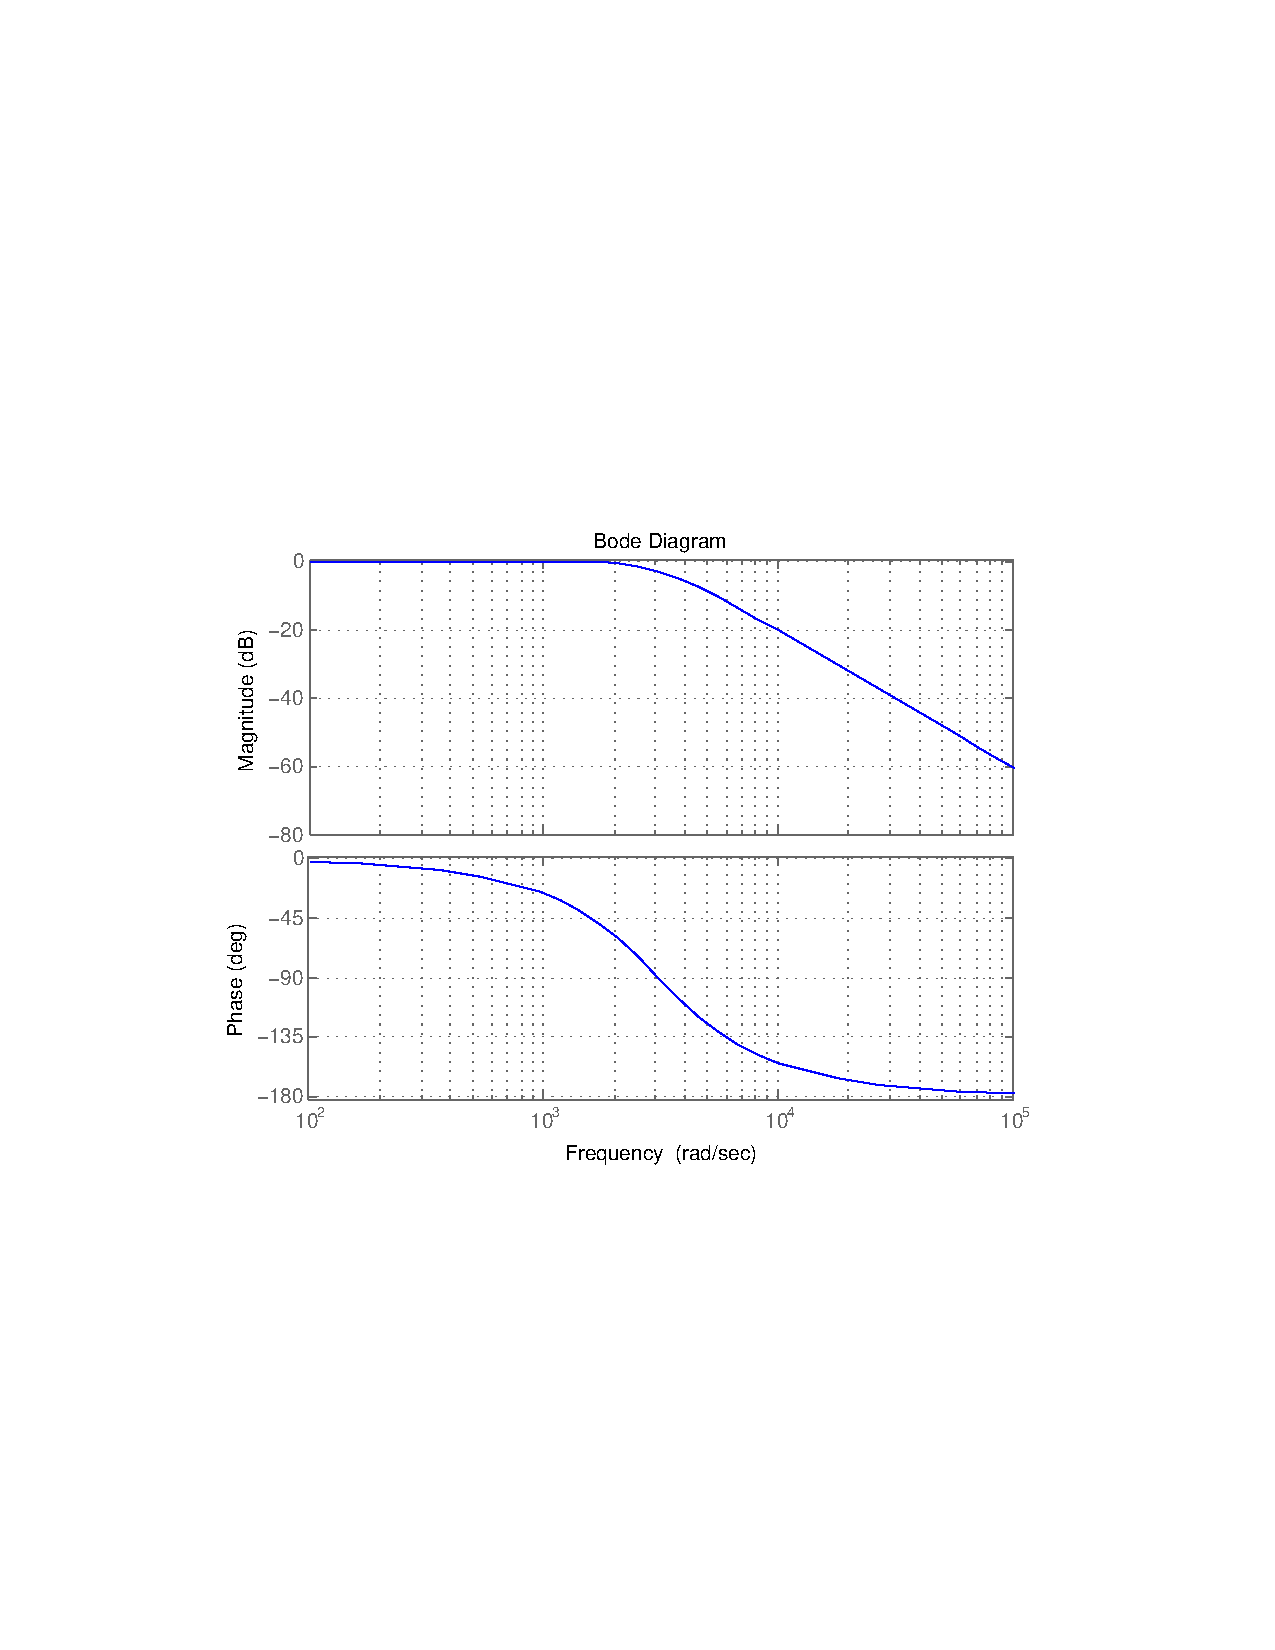
\includegraphics[scale=0.7, trim = 3.5cm 7cm 3.5cm 7cm, clip]{Bilder/butter_2} %FIXME [width=640px, height=474px]
                    \caption{Butterworth Filter 2. Ordn.}
                \end{figure}

            \end{minipage}
        
            \begin{minipage}{0.6\textwidth}
                \begin{figure}[H]
                    \label{fig:butter_2}
                    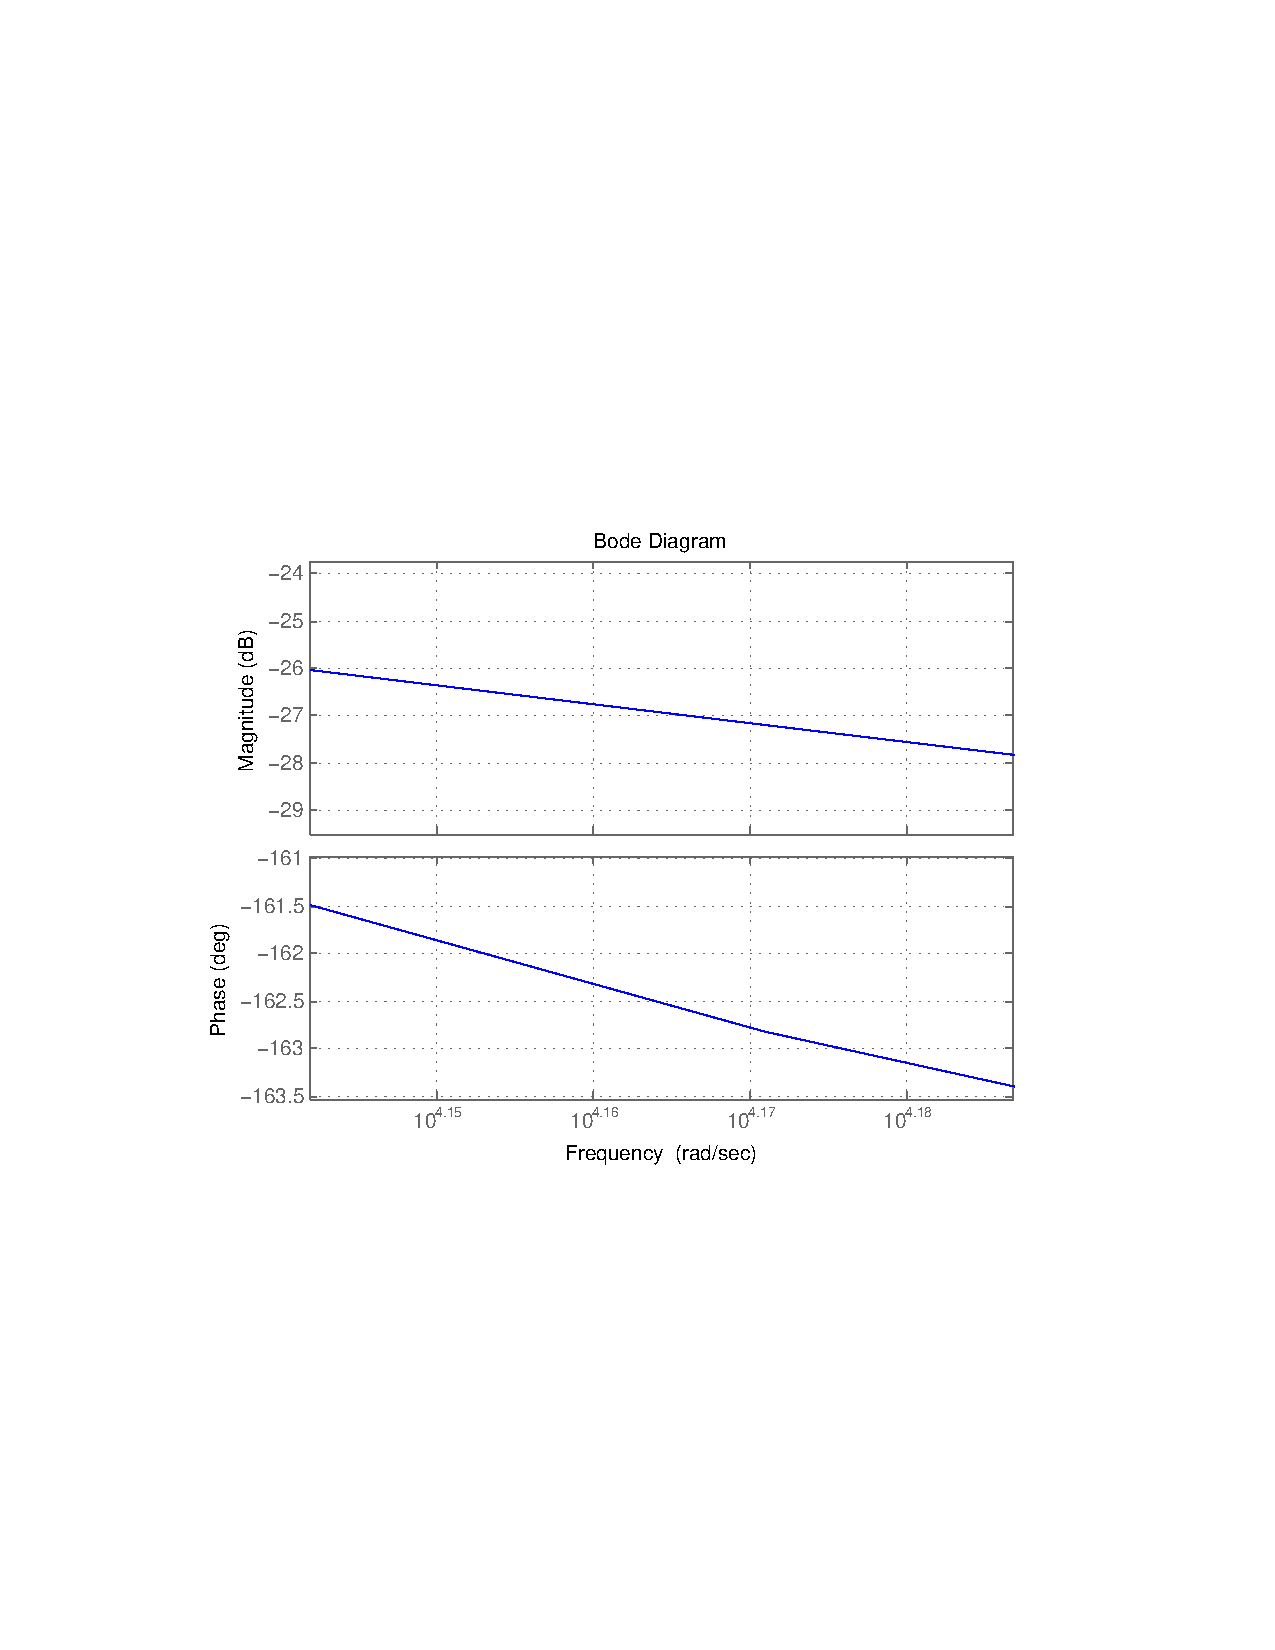
\includegraphics[scale=0.7, trim = 3.5cm 7cm 3.5cm 7cm, clip]{Bilder/butter_2_zoom} %FIXME [width=640px, height=474px]
                    \caption{In die Grafik des Filters hineingezoomt}
                \end{figure}
            \vspace{-0.4cm}
                                    
            \end{minipage}
        
        \end{tabular}
        \end{center}
            
        \vspace{1.5 cm}    
        Daraus folgt, dass $f \approx 100 kHz$.\\
        Da $f_0 < 2 \p f$ sein muss, ist die Mindestabtastrate:\\
         
        \begin{equation}
    	\begin{split}
            f_0 \approx 2 \p 100 kHz = 200 kHz
    	\end{split}
        \end{equation}
    \end{quote}




    \subsection{Tiefpassfilter 8. Ordnung}
    \begin{quote}
        
        Die Vorgehensweise beim Tiefpass 8. ordnung ist analog.
        
        
        %2 Grafiken:
        \begin{center}
        \vspace{-1.5cm}
                
        \end{center}
        \begin{tabular}{ll}
        
        \hspace{-4.5cm}
            \begin{minipage}{0.6\textwidth}
                
                \begin{figure}[H]
                    \label{fig:butter_2} 
                    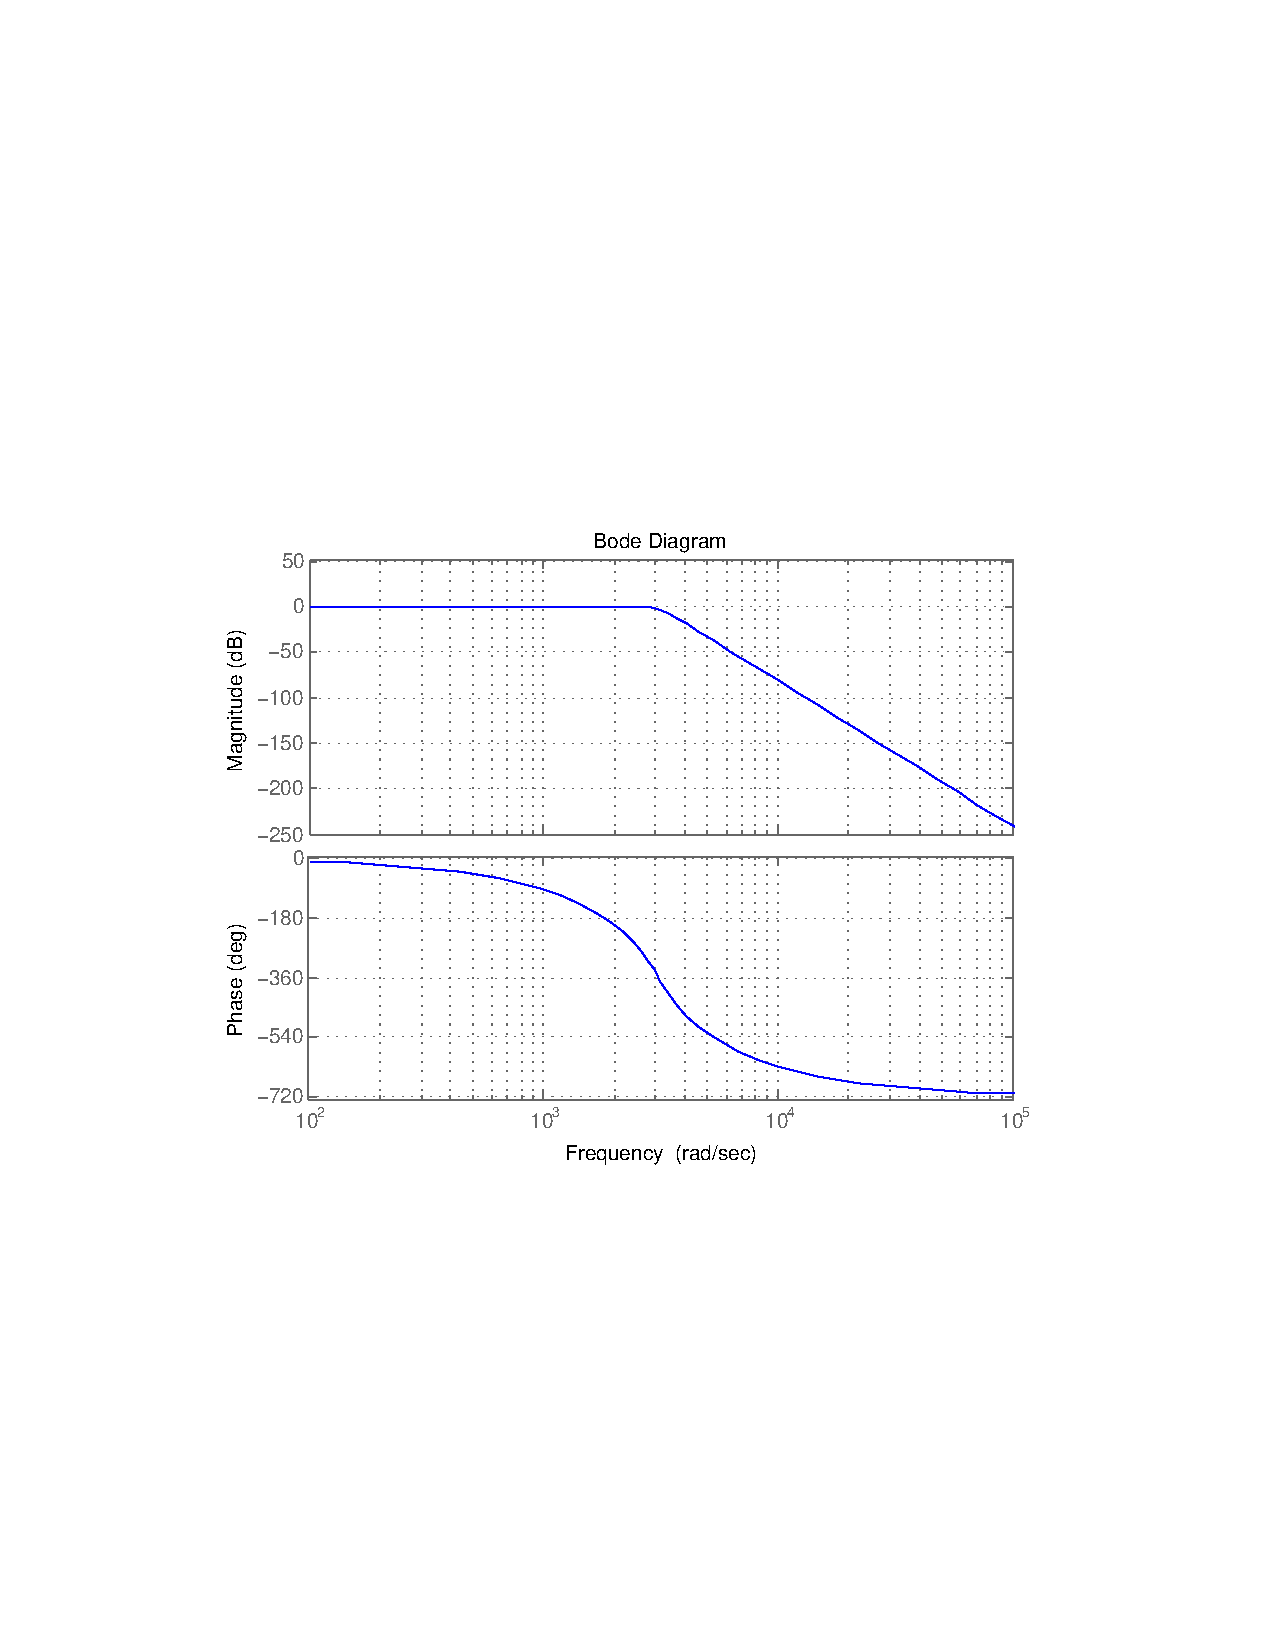
\includegraphics[scale=0.7, trim = 3.5cm 7cm 3.5cm 7cm, clip]{Bilder/butter_8} %FIXME [width=640px, height=474px]
                    \caption{Butterworth Filter 2. Ordn.}
                \end{figure}


            \end{minipage}
            
            \begin{minipage}{0.6\textwidth}
                \begin{figure}[H]
                    \label{fig:butter_2}
                    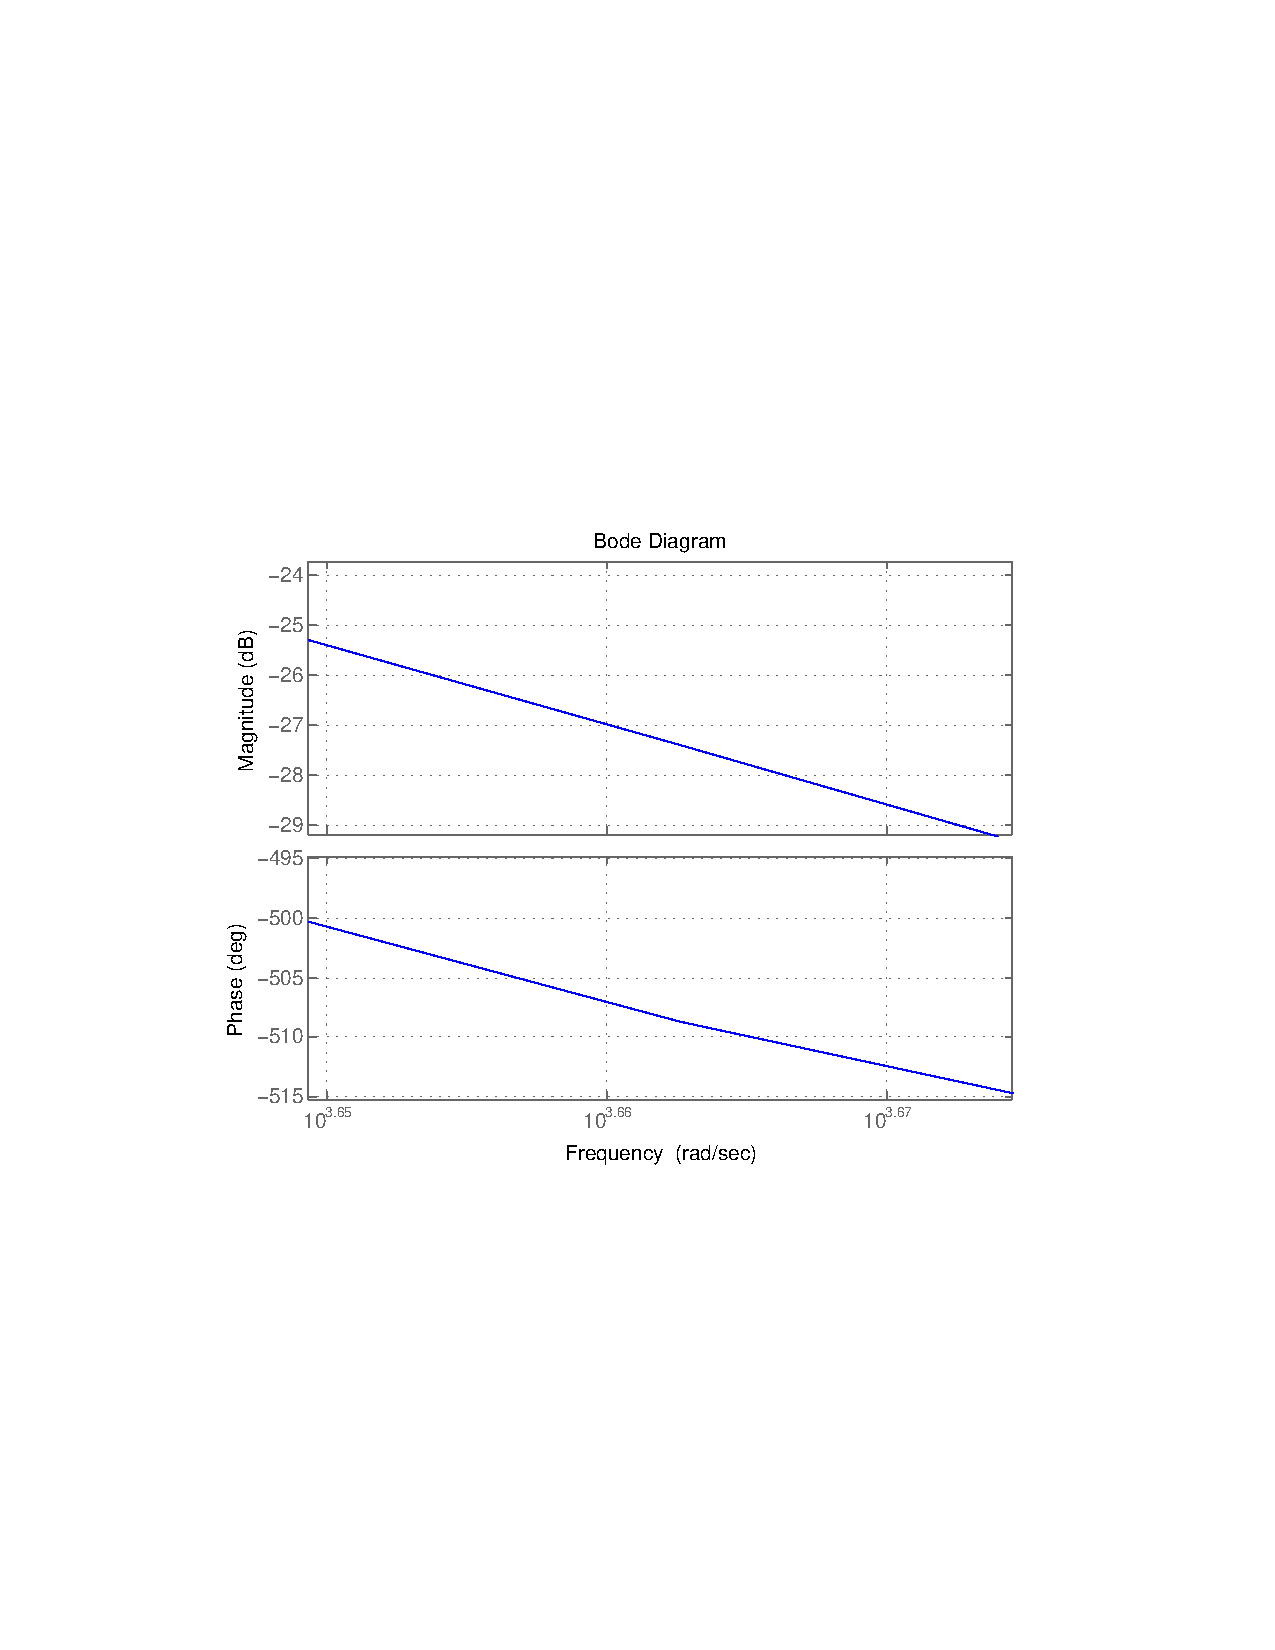
\includegraphics[scale=0.7, trim = 3.5cm 7cm 3.5cm 7cm, clip]{Bilder/butter_8_zoom} %FIXME [width=640px, height=474px]
                    \caption{In die Grafik des Filters hineingezoomt}
                \end{figure}
            \vspace{-0.4cm}
            
            \end{minipage}
        
        \end{tabular}
        \end{center}
    \end{quote}

    \begin{equation}
    \begin{split}
        f_0 \approx 2 \p 7,3 kHz = 14,6 kHz
    \end{split}
    \end{equation}
    
    
    Mit diesem Tiefpass müssten wir mit mindestens $14,6 kHz$ abtasten. Da wir in diesem Versuch aber nur eine
    Spektralanalyse bis maximal $f_m = 2 kHz$ durchführen möchten, stören uns Aliasingeffekte über $2 kHz$ nicht, weshalb
    es genügt mit $6 kHz$ ab zu tasten.
    
    
    

    
\end{quote}



\section{Praxisteil}
\begin{quote}
    
    \subsection{Ineare Regression, Steigung und Offset der ADU-Kennlinie}
    \begin{quote}
        
        \begin{figure}[H]
        \centering
            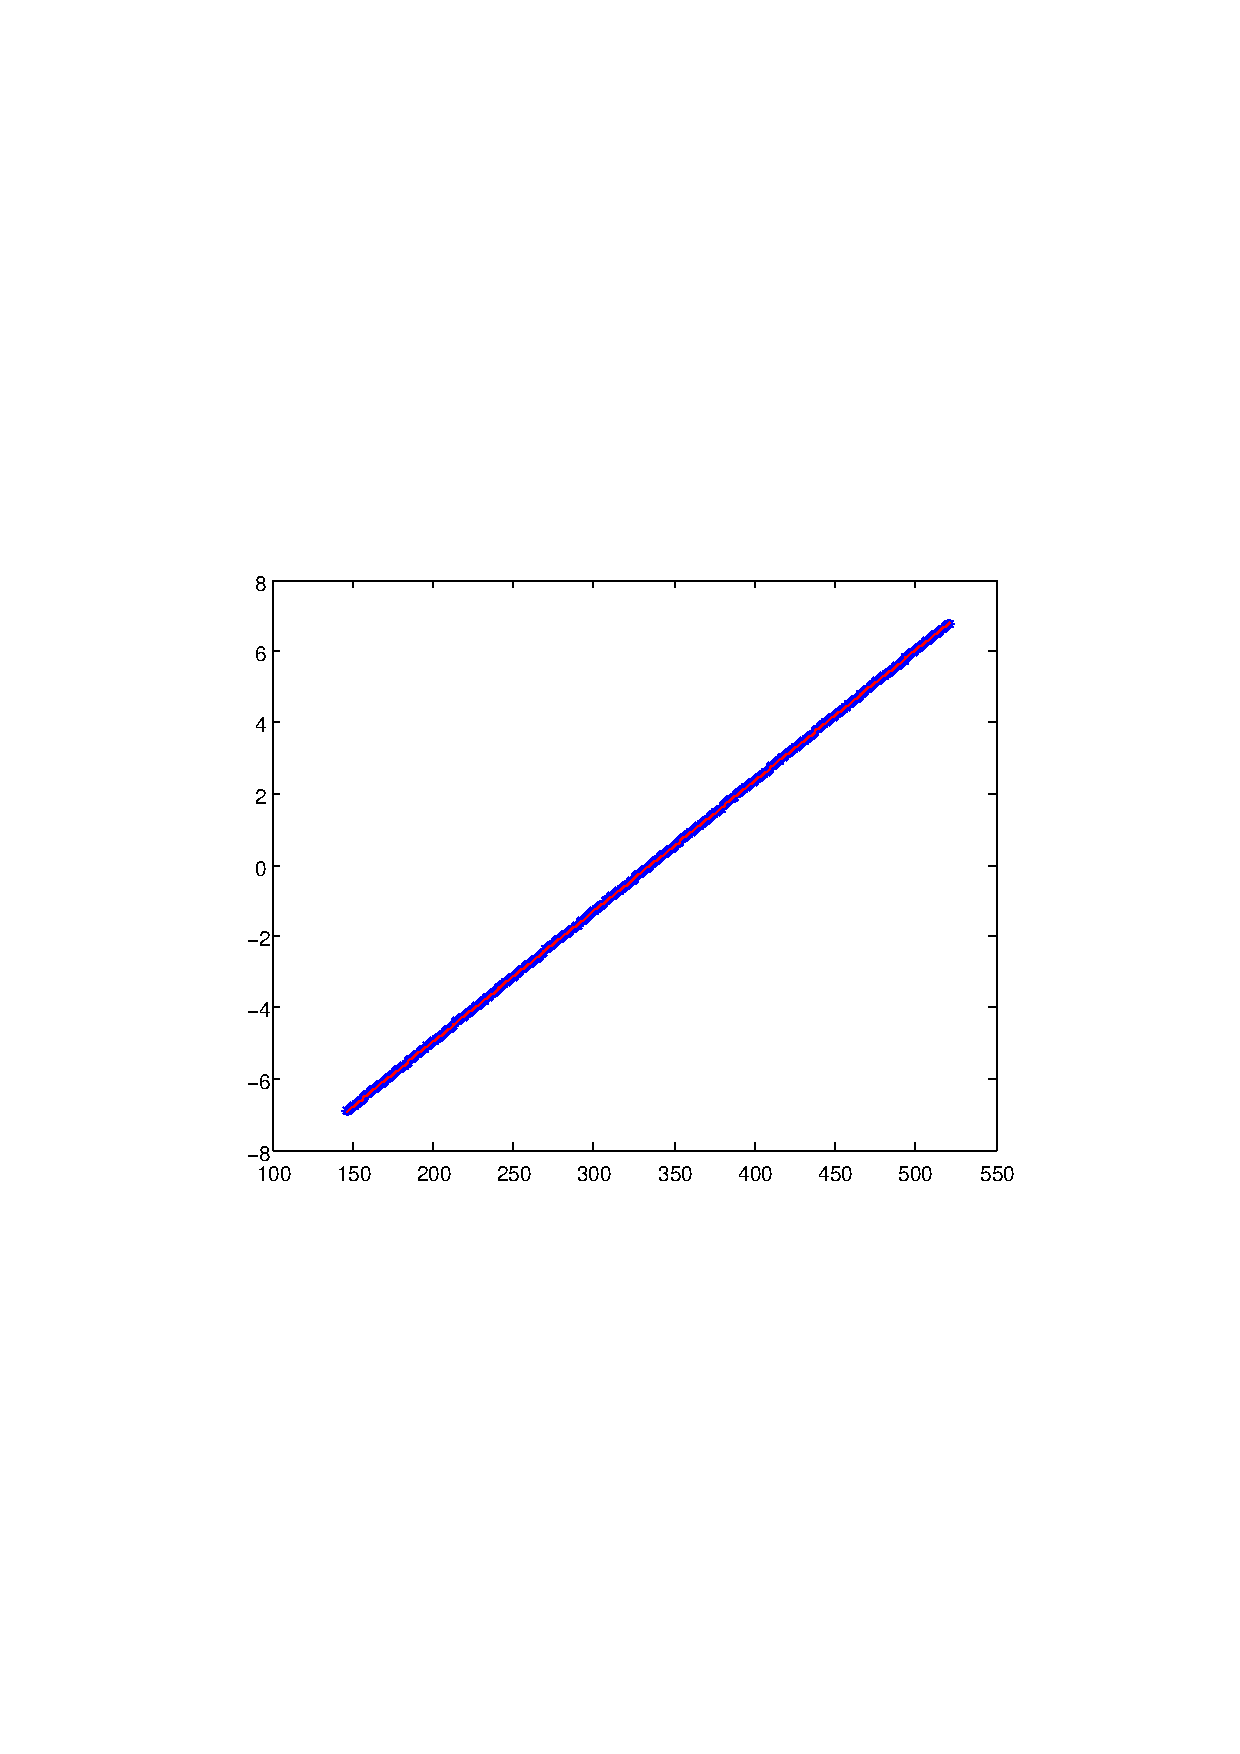
\includegraphics[scale=0.7, trim = 30mm 90mm 30mm 90mm, clip]{Bilder/ADUKennlinieplusRegr_V}
                \caption{ADU-Kennlinie + Regressionsgerade}
                \label{fig:ADUKennlinieplusRegr}
        \end{figure}
        
        Der Offset beträgt $-0.0959 V$ und die Steigung ist $0.0367$.
        
        
    \end{quote}


    \subsection{Rauschen}
    \begin{quote}
        
        \begin{figure}[H]
        \centering
            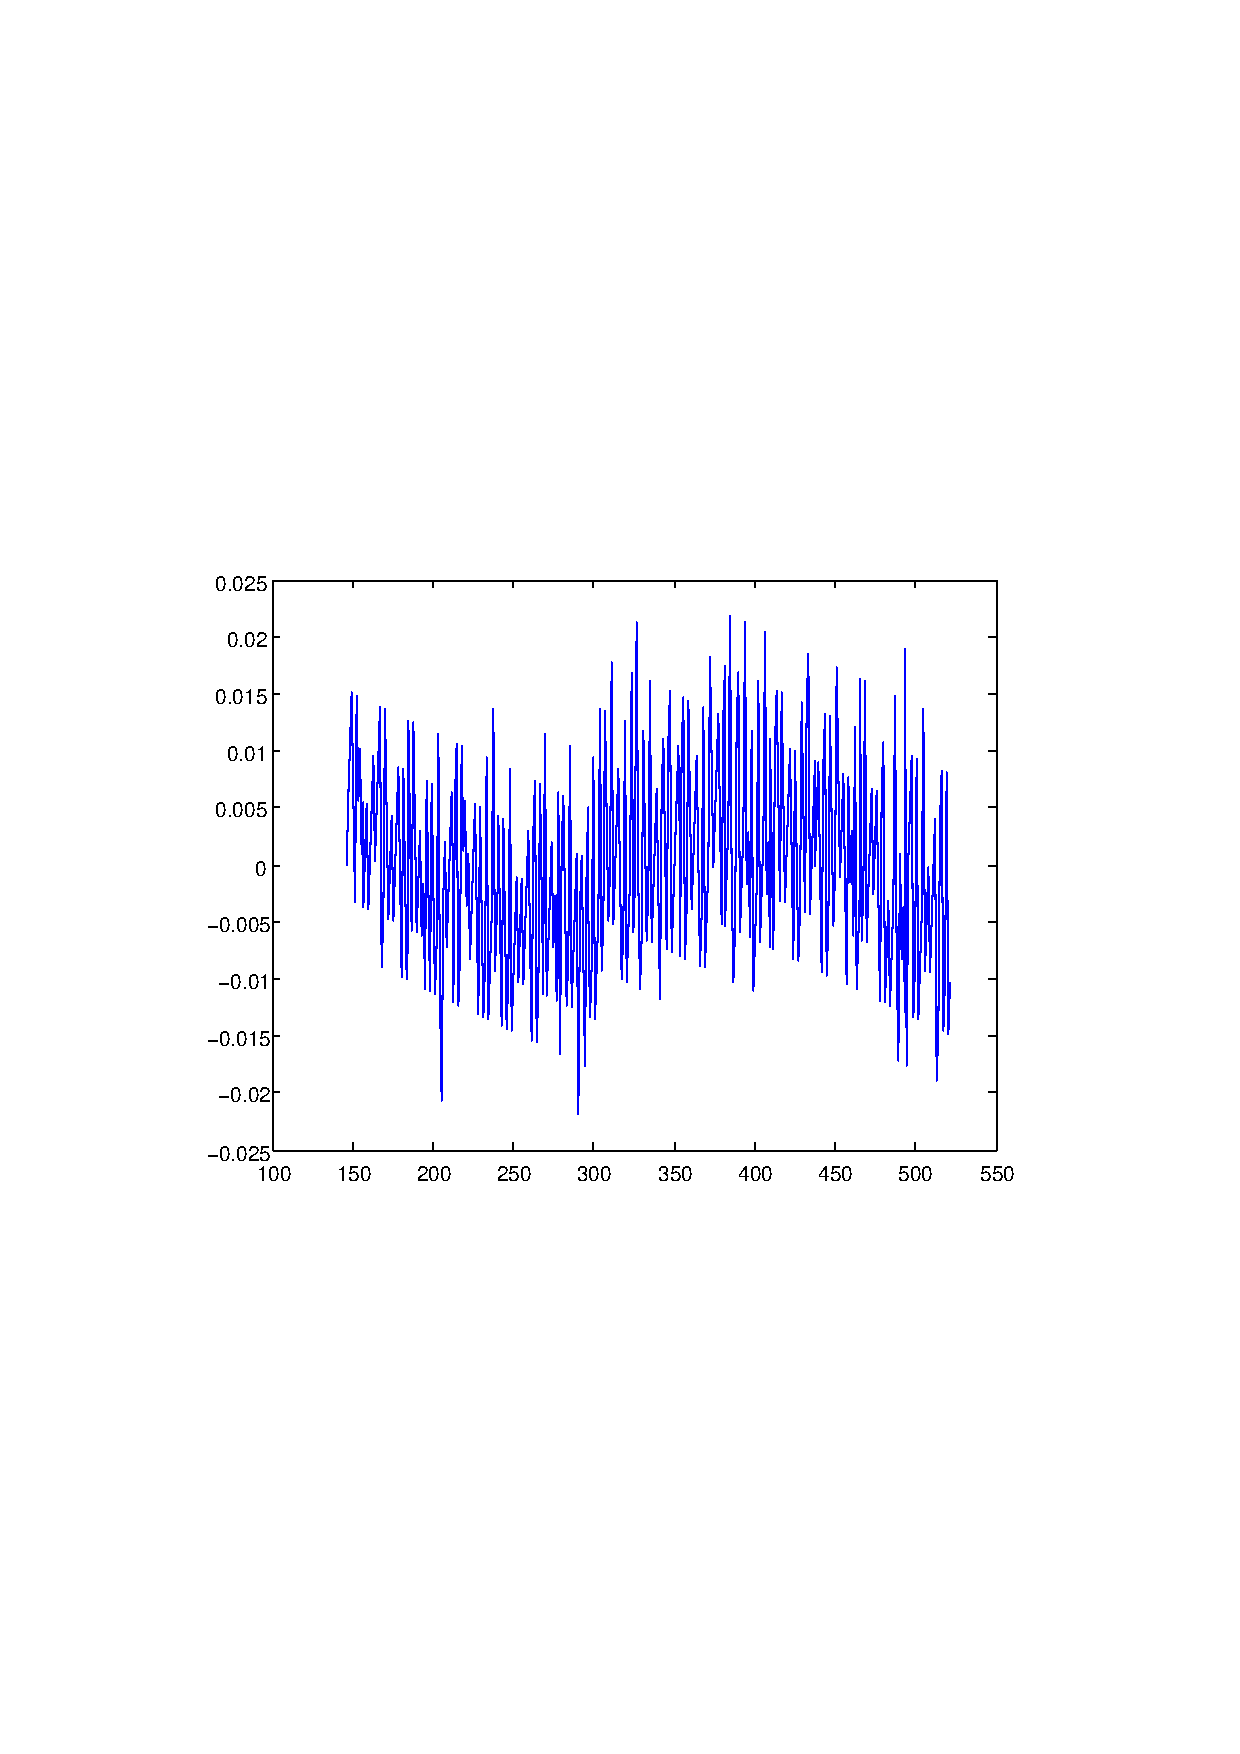
\includegraphics[scale=0.7, trim = 30mm 90mm 30mm 90mm, clip]{Bilder/Rauschen}
                \caption{Rauschen}
                \label{fig:Rauschen}
        \end{figure}
        
        Der Effektivwert des Rauschens ist $ 0.0091 V$. Das Singal- zu Rauschverhältnis beträgt $121.5515$.
        
    \end{quote}


    
    \subsection{Amplitdenfrequenzgang des Antialiasing-Filters}
    \begin{quote}
        
        \begin{figure}[H]
        \centering
            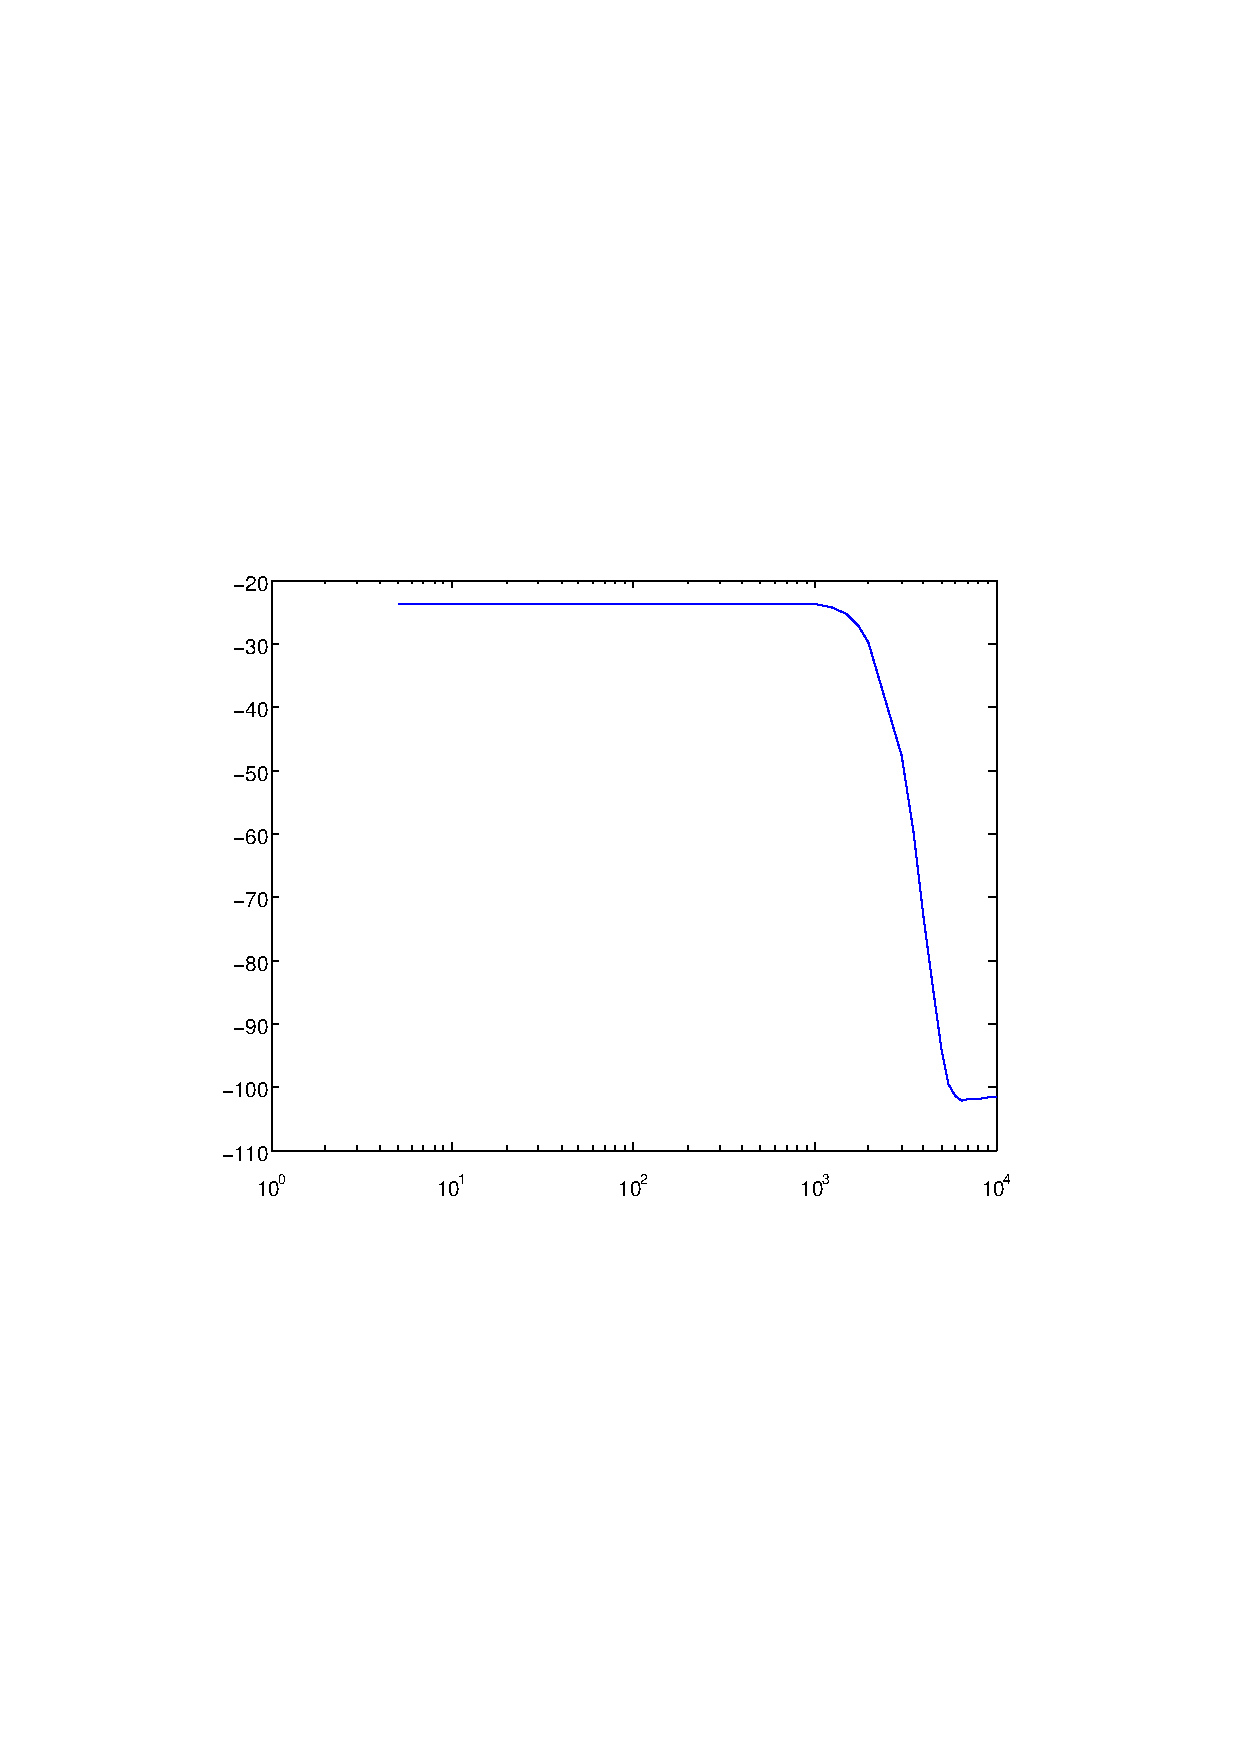
\includegraphics[scale=0.9, trim = 30mm 90mm 30mm 90mm, clip]{Bilder/realer_filter}
                \caption{Amplitdenfrequenzgang des Antialiasing-Filters}
                \label{fig:Rauschen}
        \end{figure}
        
        
        Der Amplitudenfrequenzgang des realen Filters weicht an einigen Stellen von dem des simulierten, idealen ab.\\
        Der Amplitudengang startet nicht bei $0 bB$, da in der Leitung und im Filter Verluste entstehen.\\
        Außerdem knickt der Reale Filter nicht so abrupt ab sondern hat einen weicheren Verlauf, was auf die nicht idealen
        Bauteileigenschaften zurückzuführen ist. Aus dem selben Grund ist die Steigung nicht ganz so steil wie in der
        Simulation.\\
        Schließlich wird die Dämpfung nicht unendliche groß, da der ADU sehr kleine Spannungen nicht mehr auflösen kann.
        
    \end{quote}

    
    
\end{quote}


\subsection{Matlab-Code}
    \begin{quote}
        
        \lstinputlisting[
            caption={Matlab-script},
            label=lst:Matlab]
            {./Matlab/unser_script.m}
            
            \lstinputlisting[
            caption={Matlab-script},
            label=lst:Matlab]
            {./Matlab/Code2Volt.m}


    \end{quote}






\end{document}
